% \chapter{Abordagem/Análise/Modelação}\label{cap:metodology}

% Neste capítulo espera-se uma descrição detalhada do problema e da proposta de solução. 

% No caso de projetos de desenvolvimento de software, deverá deitar-se mão dos conceitos e ferramentas de Análise/Modelação estudadas durante o curso (por exemplo, diagramas UML ou outra linguagem gráfica). Deve-se indicar explicitamente as tarefas a desempenhar pelo sistema, e os atores que interagem com o mesmo. A descrição deve ter suficiente detalhes  para perceber as dificuldades associadas à resolução do problema.


\chapter{Methodology}\label{cap:metodology}
A seção de metodologia explora uma abordagem para o desenvolvimento do software, iniciando com a definição dos requisitos, passando pela definição do método de recebimento dos dados, e a seleção das tecnologias. O processo de desenvolvimento incorpora a criação de histórias de usuário, organizadas em um quadro Kanban para gerenciamento de tarefas, e à configuração dos repositórios. A documentação e reuniões regulares que acompanham o progresso, são uma constante em todas as fases para garantir que o projeto está ocorrendo como o esperado.

\section[Definição dos requisitos]{Definição dos requisitos}\label{sec:req}
A definição precisa dos requisitos é fundamental para garantir que o sistema desenvolvido atenda às necessidades e objetivos do projeto de maneira ágil \cite{asghar2016role}. Os requisitos desse projeto foram classificados nas categorias funcionais e não funcionais, para garantir uma compreensão completa do que é esperado do sistema.

\subsection[Requisitos Funcionais]{Requisitos Funcionais}
Os requisitos funcionais desempenham um papel fundamental no desenvolvimento de sistemas, definindo as funções que um sistema ou componente de software deve ser capaz de executar. Em essência, eles fornecem uma descrição das interações que o sistema terá com seus usuários ou com outros sistemas, especificando os serviços que o sistema deve fornecer.

Para garantir eficácia, os requisitos funcionais devem ser claramente definidos, sem ambiguidades, e serem mensuráveis, rastreáveis, completos e consistentes. Além disso, eles devem ser definidos levando em consideração as necessidades e objetivos do projeto, garantindo que o sistema desenvolvido seja não apenas tecnicamente sólido, mas também útil e relevante para seus usuários finais.

Dentro do contexto do sistema desenvolvido, está listado abaixo os requisitos funcionais do sistema e sua descrição, de forma a deixar claro, de forma funcional, o que o sistema deve fazer.

\subsubsection{FR1 - O sistema deve permitir que um usuário acesse o sistema de forma segura com um email e senha}
Dado que o sistema é para a visualização dos dados de operação de uma industria de estampagem, as informações disponibilizadas devem ser acessadas apenas por usuários previamente autorizados.

\subsubsection{FR2 - O sistema deve permitir que um usuário veja as suas informações pessoais que são armazenadas nos sistema}
Cada usuário que tiver acesso ao sistema terá registrado nele alguns de seus dados pessoais, como e-mail, cargo e tipo de acesso. Portanto, cada usuário deve ter acesso a suas informações pessoais que estão salvas no sistema.

\subsubsection{FR3 - O sistema deve exibir em tempo real os valores lidos pelos sensores em cada uma das máquinas}
Ao receber os dados enviados pelos sensores, os sistema deve exibir em tela os valores lidos, separado por tipo de sensor e máquina. 

\subsubsection{FR4 - O sistema deve armazenar um valor máximo ideal para cada para tipo de sensor utilizado}
Cada sensor deverá ter um valor máximo ideal para o funcionamento. Ele servirá de parâmetro para entender se o valor lido pelo sensor indica um bom ou mal funcionamento da máquina.

\subsubsection{FR5 - O sistema deve identificar sempre que um valor lido pelo sensor não estiver abaixo do valor ideal}
Esse requisito refere-se à capacidade do sistema de detectar, de forma automática, toda vez que o sensor indicar um valor que não esteja abaixo do limite pré definido. Isto é, se o valor ideal for X, e o sensor ler um valor maior ou igual a X, o sistema reconhecerá esta situação.

\subsubsection{FR6 - O sistema deve registrar sempre que um valor lido pelo sensor não estiver de acordo com o valor ideal}
Esse requisito implica que o sistema deve manter um registro de todos os momentos em que o valor detectado pelo sensor não estiver abaixo do valor ideal armazenado.

\subsubsection{FR7 - O sistema deve mostrar em tela quando um valor lido pelo sensor não estiver abaixo do ideal}
Sempre que o sensor detectar um valor abaixo do padrão ideal, o sistema deverá exibir um alerta na interface de forma que fique sempre visível para o usuário.

\subsubsection{FR8 - O sistema deve mostrar no formato de notificação os registros de não funcionamento abaixo do valor ideal}
Este requisito estabelece que o sistema deve apresentar aos usuários na forma de notificações quando o sensor ler um valor acima do ideal, para possibilitar que os usuários sejam informados, mesmo que posteriormente, sempre que um alerta for identificado.

\subsubsection{FR9 - O sistema deve permitir que o usuário marque uma notificação como lida, de forma que ela não apareça novamente}
Após ser notificado, os usuários deverão ter a capacidade de marcar essa notificação como "lida", garantindo que a mesma informação não continue a ser exibida repetidamente.

\subsubsection{FR10 - O sistema deve exibir gráficos mostrando os valores lidos pelos sensores nos dias anteriores de forma agregada, separando por máquinas}
Esse requisito assegura que os usuários possam visualizar, por meio de representações gráficas, as leituras dos sensores de dias anteriores de forma agregada. Estes gráficos devem ser categorizados por máquina, proporcionando uma análise detalhada do desempenho de cada equipamento ao longo do tempo.

\subsubsection{FR11 - O sistema deve exibir nos gráficos uma análise estatística do funcionamento das máquinas, junto com o valor máximo de funcionamento ideal}
Os gráficos devem oferecer uma análise estatística, mostrando os indicadores estatísticos dos dados agregados média, mediana, percentil 75 e média removendo os outliers. Juntamente com isso, o gráfico também mostrará o valor ideal, servindo como uma referência para avaliar o desempenho.

\subsubsection{FR12 - O sistema deve permitir filtrar as informações exibidas em tela por máquinas}
Os usuários devem ter a flexibilidade de selecionar e visualizar informações específicas para determinadas máquinas, permitindo que eles se concentrem em equipamentos específicos conforme a necessidade.

\subsubsection{FR13 - O sistema deve permitir filtrar os gráficos exibidas em tela por data}
O sistema deve oferecer a capacidade de os usuários filtrarem as exibições gráficas por datas específicas, permitindo análises temporais detalhadas e comparações entre diferentes períodos.

\subsubsection{FR13 - O sistema deve exibir os gráficos de parada das máquinas de forma a exemplificar a exibição desses dados}
O sistema deve mostrar as paradas de máquina de acordo com os dados passados pelas planilhas com os dados. Dessa forma poderá ser exemplificado como ficaria as informações de parada das maquinas caso o sistema recebesse essas informações.


\subsection[Requisitos Não Funcionais]{Requisitos Não Funcionais}\label{ssubec:reqNfuctional}
Requisitos não funcionais são especificações que determinam as características de desempenho, usabilidade, confiabilidade e outras propriedades que o sistema deve possuir, ao invés de comportamentos específicos que ele deve demonstrar. Enquanto os requisitos funcionais descrevem o que um sistema deve fazer, os requisitos não funcionais especificam como o sistema deve realizar essas funções.

Estes requisitos são cruciais para garantir a satisfação do usuário e a eficácia operacional do sistema, desempenhando um papel fundamental na qualidade e na operação geral de um produto de software.

Os requisitos não funcionais podem ser de vários tipos, como usabilidade, desempenho, segurança, disponibilidade, manutenção e confiabilidade. Dentro do contexto do sistema desenvolvido, está listado abaixo os requisitos não funcionais do sistema e sua descrição, de forma a deixar claro o que foi levado em consideração no momento de desenvolver cada uma das funcionalidades do sistema.

\subsubsection{NFR1 - Disponibilidade}
O sistema deve possuir mecanismos de reconexão automática que se ativam quando problemas de conexão ou recebimento de dados dos sensores forem detectados, garantindo assim a continuidade no recebimento dos dados.

\subsubsection{NFR2 - Segurança no acesso}
O sistema deve implementar controles de acesso para que somente colaboradores autorizados tenham permissão para acessar os dados e funcionalidades pertinentes ao seu papel.

\subsubsection{NFR3 - Segurança na rede}
Para garantir a segurança da transmissão de dados, a conexão ao sistema deve ser estabelecida utilizando o protocolo \gls{HTTPS}, que incorpora a camada de segurança \gls{TLS}, protegendo assim os dados contra intercepções e alterações.

\subsubsection{NFR4 - Transmissão em tempo real}
O sistema deve processar e transmitir os dados enviados pelos sensores em uma arquitetura baseada em streaming. O atraso entre o envio do dado pelo sensor e sua visualização pelo usuário final deve ser inferior a três segundos.

\subsubsection{NFR5 - Modularidade}
A arquitetura do sistema deve ser modular, possibilitando a integração e a adição de novos componentes ou funcionalidades de maneira eficiente e sem comprometer o funcionamento das partes já existentes.


\subsubsection{NFR6 - Manutenibilidade}
Priorizando a longevidade e facilidade de manutenção, o sistema deve ser desenvolvido seguindo boas práticas de programação e modularização do sistema. Isso facilitará futuras modificações, expansões e a correção de eventuais problemas.

\subsubsection{NFR7 - Escalabilidade de sensores e máquinas}
O design do sistema deve ser capaz de lidar com um crescente volume de sensores e máquinas, garantindo que não haja degradação de performance ou falhas quando a demanda por recursos aumentar.

\subsubsection{NFR8 - Portabilidade}
O sistema deve garantir compatibilidade com os principais navegadores web disponíveis no mercado. Além disso, a interface de usuário deve se adaptar bem em telas maiores como televisões, permitindo que o dashboard seja visualizado de forma clara em diferentes ambientes da fábrica.

\subsubsection{NFR9 - Usabilidade}
A interface do sistema e seus componentes devem ser projetados considerando princípios fundamentais de design de interação, garantindo que os usuários possam compreender e interagir com o sistema de maneira intuitiva e eficiente.


\section[Método de coleta e armazenamento de dados]{Método de coleta e armazenamento de dados}
%como que seria feito o recebimento e o armazenamento dos dados
%- Recebimento dos dados pelo protocolo feito pelo outro professor
%- protocolo esse que decodifico as informações e disponibilizo para uso

%TODO 10Artigo Referencia para o outro projeto com os sensores e protocolos - Referenciar o Attract 
Dentro do contexto do projeto, a forma como os dados dos sensores são coletados e armazenados influenciam muito no funcionamento do sistema, pois é a partir deles que todo o sistema é estruturado. Dessa forma foi utilizado como base um protocolo desenvolvido em outro projeto dentro do mesmo contexto do \texttt{Projeto Attract}, que transmite todas as informações necessárias para o contexto desse projeto. Dentro do sistema em questão, ficou a responsabilidade de implementar o decodificador para o determinado protocolo.

O formato do protocolo é estruturado de forma a representar as informações pertinentes à máquina, ao tipo de comunicação, ao sensor e ao significado dos dados transmitidos, seguindo o seguinte formato:

\subsubsection{Machine ID (2 bytes)}

O campo \textit{Machine ID} é responsável por identificar a máquina em questão e está dividido em dois subcampos:

\begin{itemize}
    \item \textbf{High (bytes de ordem superior)}: Representa o tipo da máquina. Exemplos de valores possíveis são: prensa, torno, robot, tapete, entre outros.
    \item \textbf{Low (bytes de ordem inferior)}: Identifica o número da máquina.
\end{itemize}

\subsubsection{Type (1 byte)}

O campo \textit{Type} indica o tipo de mensagem e pode assumir os seguintes valores:
\begin{enumerate}
    \item Publish
    \item Request to publish
\end{enumerate}

\subsubsection{Sensor ID (2 bytes)}

O campo \textit{Sensor ID} fornece detalhes sobre o sensor que está transmitindo os dados:

\begin{itemize}
    \item \textbf{High (bytes de ordem superior)}: Representa a quantidade física sendo medida, como temperatura, velocidade, pressão, força, entre outros.
    \item \textbf{Low (bytes de ordem inferior)}: Indica o número do sensor.
\end{itemize}

\subsubsection{Meaning of Data (2 bytes)}

O campo \textit{Meaning of Data} fornece informações sobre o tipo e significado dos dados:

\begin{itemize}
    \item \textbf{High (bytes de ordem superior)}: Tipo dos dados:
    \begin{enumerate}
        \item Not defined
        \item Normal
        \item Raw data
        \item Alarm
    \end{enumerate}
    \item \textbf{Low (bytes de ordem inferior)}: Significado dos dados, que varia de acordo com o equipamento. Exemplos incluem:
    \begin{itemize}
        \item Oil critical temperature
        \item Check oil temperature
        \item Oil pressure
    \end{itemize}
\end{itemize}

\subsubsection{Length (2 bytes)}

O campo \textit{Length} indica o número de bytes subsequentes no pacote.

\subsubsection{Data}

Este campo representa os dados transmitidos pelo sensor. A especificação exata do que os dados representam deve ser definida e normalizada, conforme indicado pela notação (*).


\section[Processo de desenvolvimento do software]{Processo de desenvolvimento do software}
Com a definição clara dos requisitos do sistema e da forma como os dados lidos pelos sensores são transmitidos, foi definido o processo de como o projeto seria desenvolvido. Esse processo de desenvolvimento passa pela definição das histórias de usuário, organização das atividades, organização da documentação, configuração dos repositórios no GitHub e reuniões periódicas com o professor orientador e com a empresa para discutir o andamento.

\subsection{Histórias de Usuário}
No desenvolvimento ágil de software, uma das abordagens mais centradas no usuário entendimento das funcionalidades do sistema e dos requisitos é a utilização de \textit{histórias de usuário}. Estas são descrições curtas, simples e informais do ponto de vista de um usuário final, capturando o que eles necessitam ou desejam fazer no software \cite{lucassen2015forging}.

A estrutura típica de uma história de usuário é: "Como [tipo de usuário], eu quero [uma ação] para que [um benefício/resultado]". Esta estrutura ajuda a manter o foco nas necessidades e desejos do usuário, em vez de mergulhar prematuramente em soluções técnicas ou detalhes de implementação.

Além de serem uma ferramenta de comunicação entre os desenvolvedores e os stakeholders, as histórias de usuário facilitam a priorização das tarefas, ajudam na criação de critérios de aceitação e fornecem uma base para discussões interativas durante as reuniões de revisão e planejamento.

Em suma, as histórias de usuário servem como um meio eficaz de traduzir requisitos complexos em tarefas gerenciáveis e centradas no usuário, garantindo que o produto final atenda às expectativas e necessidades dos seus utilizadores.

Com essa definição de historias de usuário, foi definido os seguintes itens que traduzem os requisitos em tarefas para o desenvolvimento do projeto:


\begin{enumerate}
    \item As a user, I must be able to log in with my credentials to use the system.
    \item As a user, I should be able to view my personal information on a profile page to manage the data the system holds about me.
    \item As a user, I should be able to view in real-time values of the machines to detect relevant variations in operation more quickly.
    \item As a user, I should be able to view the historical values of the sensors aggregated in charts of the machines to monitor the status over time.
    \item As a user, I should be able to filter the dashboard information by machine and by date to view data according to my needs.
    \item As a user, I should be alerted when a sensor reads a value that exceeds the ideal parameter so I can take necessary actions as quickly as possible.
    \item As a user, I should be able to view system notifications to be alerted about machine operation alerts.
    \item As a user, I should be able to view the machine downtime records for a better and more organized view of the recorded machine downtimes.
    \item As a user, I should be able to view the system information (dashboards) on different screen sizes so that I can display the information in different contexts.
\end{enumerate}

Cada uma dessas historias de usuário foi detalhada melhor na organização das tarefas, incluindo uma descrição mais completa, possíveis regras de negócio, quais requisitos, funcionais e não funcionais, ela se referencia, e também critérios de aceite. A organização das atividades está detalhada na seção \ref{sec:taskOrganization}.


\subsection{Organização das tarefas}\label{sec:taskOrganization}
O método Kanban, originário do sistema Toyota de produção, tornou-se uma ferramenta popular e eficaz para gerenciamento e organização de fluxos de trabalho. A palavra "Kanban" é de origem japonesa e pode ser traduzida como "cartão visual" ou "sinalização". No contexto de gestão de projetos, Kanban refere-se a um sistema visual de gestão que destaca o fluxo de trabalho e as tarefas em diferentes estágios de processo. A essência do Kanban é visualizar todo o fluxo de trabalho, desde as tarefas que ainda não foram iniciadas até aquelas que foram concluídas. Esta visualização permite identificar gargalos e ineficiências, otimizando assim o processo \cite{ghani2015agile}. Para a organização das atividades desse projeto, o método Kanban foi adotado como uma estratégia para garantir uma progressão eficiente e sistemática do trabalho.

Para a implementação do método Kanban, foi escolhido o Notion como ferramenta. A escolha deste software deve-se à sua flexibilidade e capacidade de personalização, permitindo a criação de um board Kanban que se adapta especificamente às necessidades do projeto \cite{notionProjectManagement}. Além disso, o Notion oferece uma interface intuitiva para a construção documentação, que está melhor detalhada na seção \ref{sec:documentation}.

O board Kanban foi estruturado em cinco colunas, cada uma representando um estágio distinto no fluxo de trabalho:

\begin{itemize}
    \item \textbf{Backlog:} Esta coluna contém todas as tarefas e atividades identificadas, mas que ainda não foram iniciadas. É um repositório de tudo o que precisa ser feito, mas que ainda não tem uma data definida para começar.
    \item \textbf{To Do:} As tarefas que estão nesta coluna estão prontas para serem iniciadas. Elas foram retiradas do Backlog, detalhadas e têm prioridade para serem iniciadas em breve.
    \item \textbf{Stopped:} Aqui estão as tarefas que foram iniciadas, mas por algum motivo tiveram que ser interrompidas, desde mudanças de prioridade, necessidade de alguma valição ou limitação técnica.
    \item \textbf{In Progress:} Esta coluna contém as tarefas que estão atualmente em execução. A movimentação para esta coluna indica que o trabalho está ativamente sendo feito na tarefa.
    \item \textbf{Done:} Assim que é finalizado o desenvolvimento de uma tarefa ela é dada como concluída, e portanto, movida para esta coluna. Representa o sucesso na finalização da atividade, e serve como um registro de todos os itens concluídos.
\end{itemize}

A estruturação destas colunas oferece uma visão clara do status de cada atividade e ajuda a identificar rapidamente onde estão os gargalos, facilitando a tomada de decisões e a priorização das tarefas.

\begin{figure}[htbp]
	\centering
	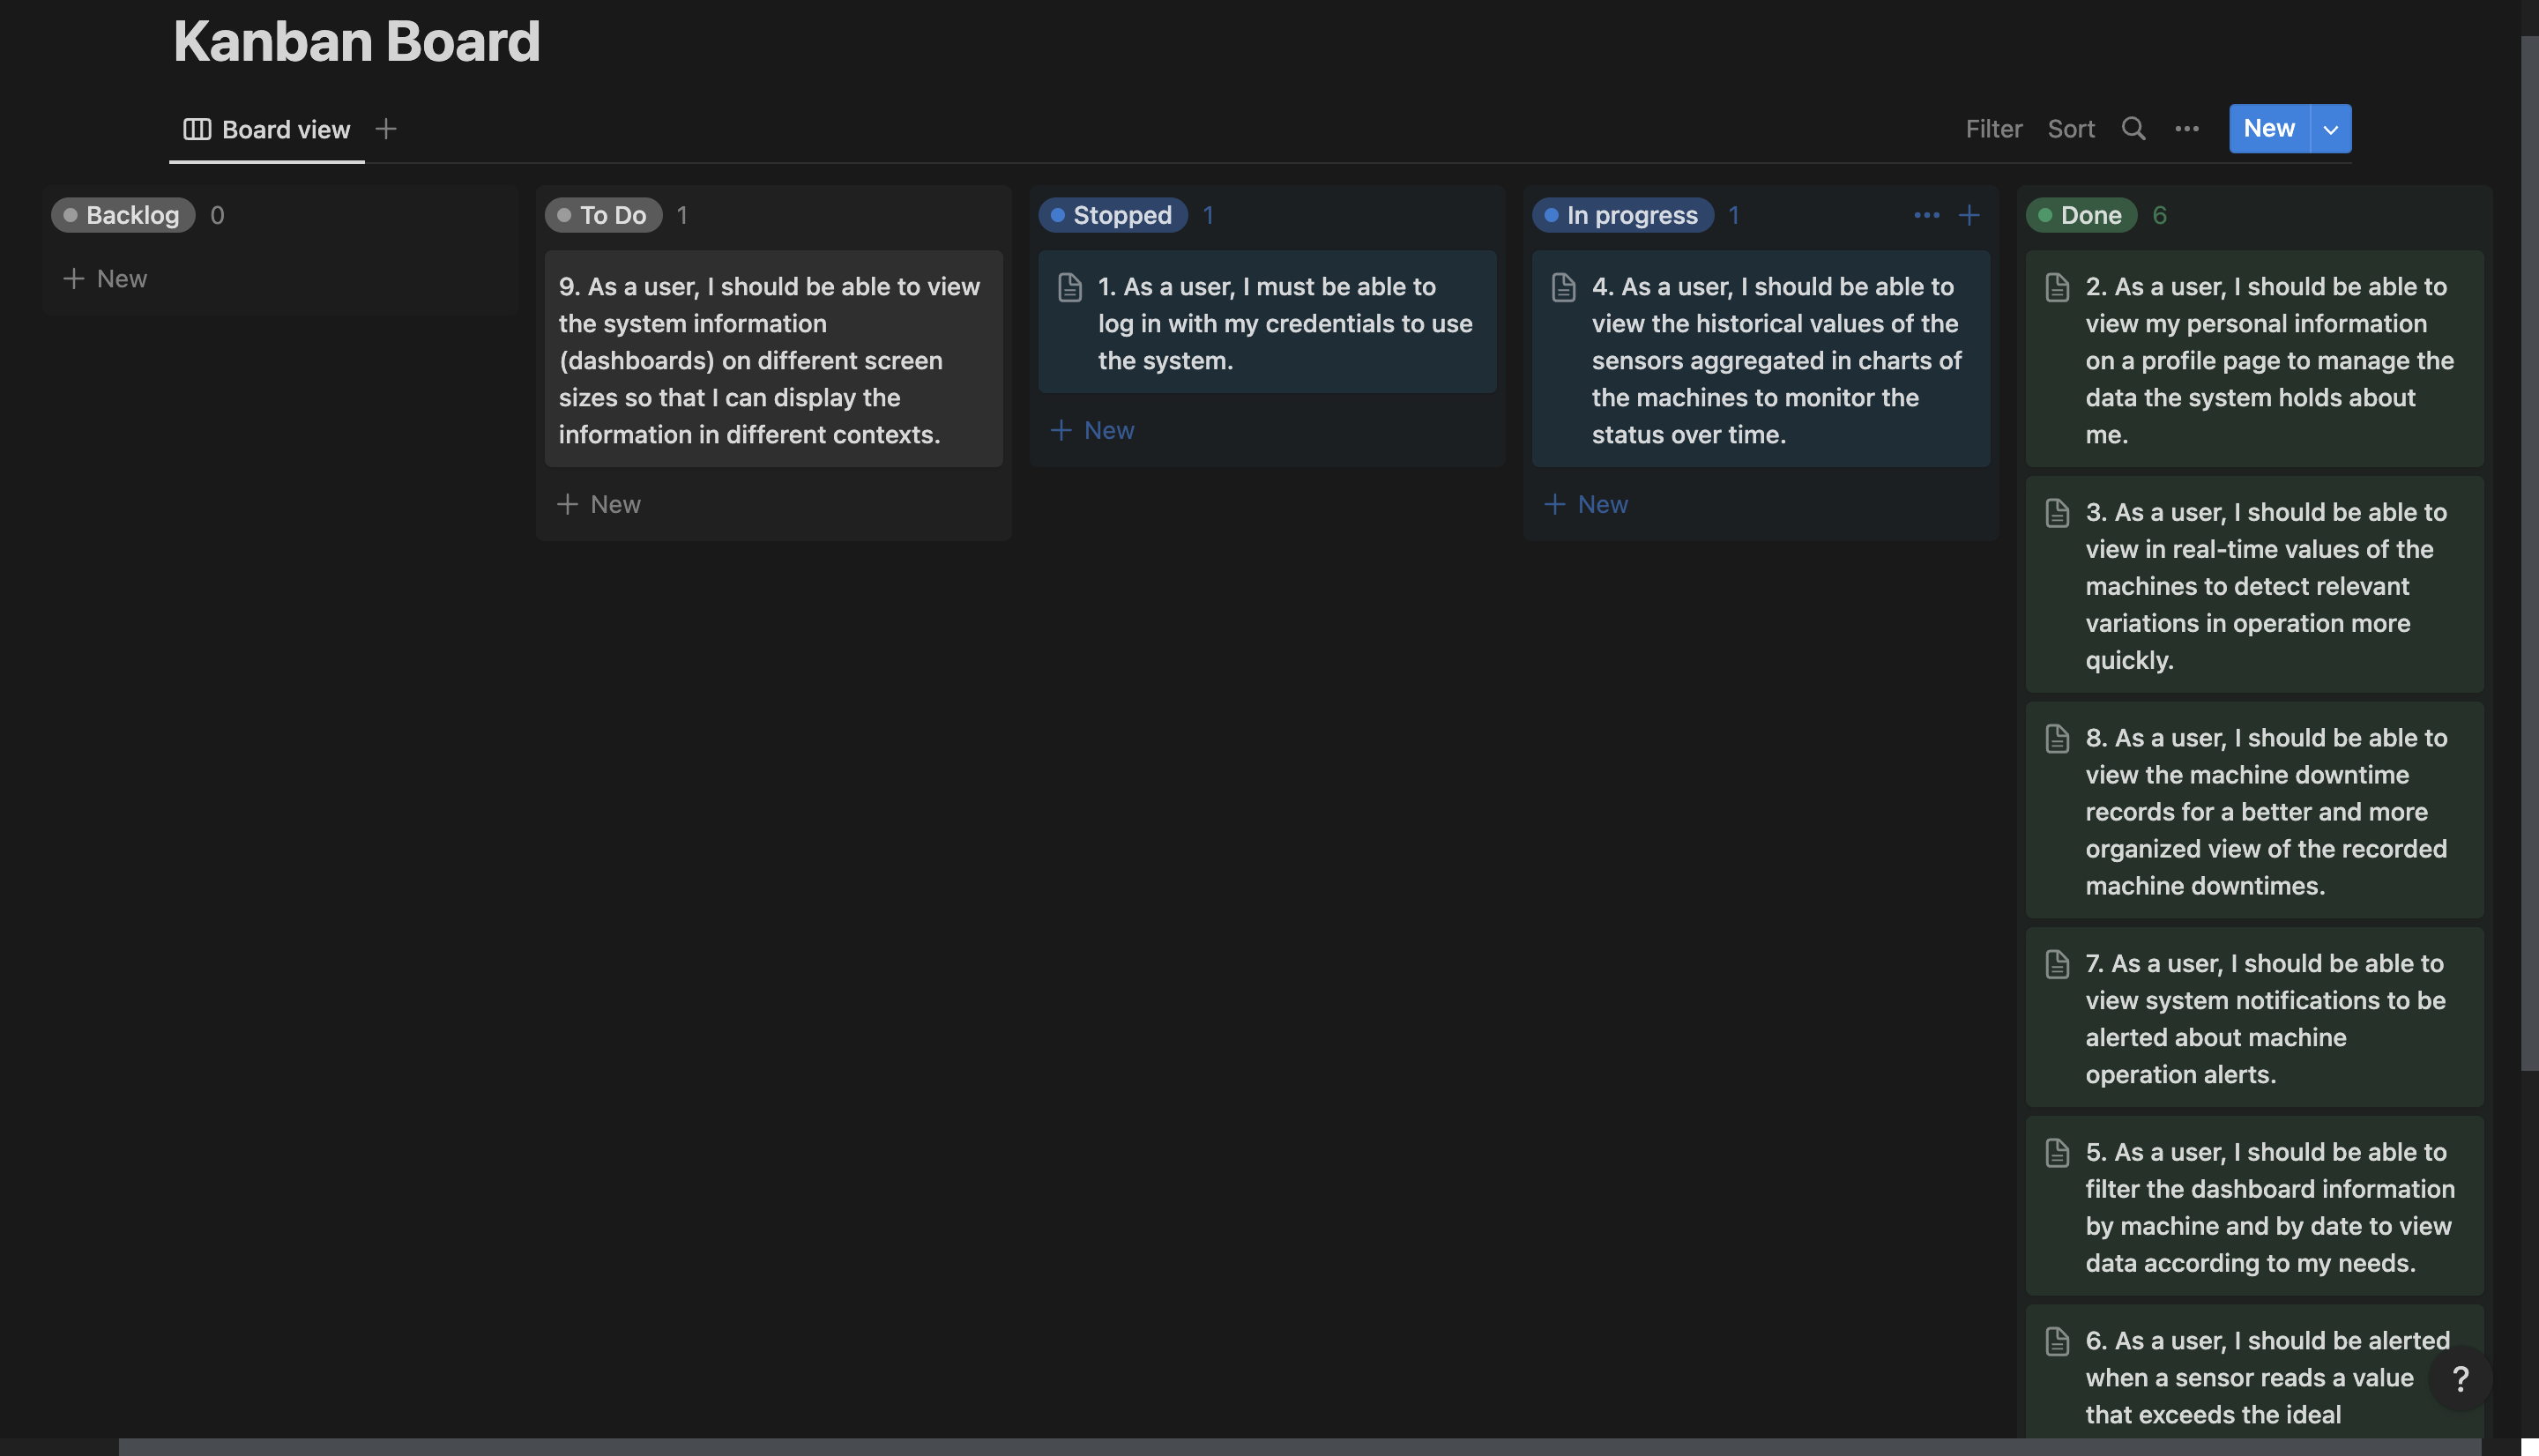
\includegraphics[width=\textwidth]{images/kanban_board}
	\caption{Board Kanban used to manager the tasks.}
	\label{fig:BoardKanban}
\end{figure}

A fim de definir melhor a implementação de cada história de usuário, cada card no board Kanban foi detalhado com uma descrição que inclui regras de negócio relevantes, referências a requisitos funcionais e não funcionais, critérios de aceitação e sub-tarefas. Antes que uma história de usuário possa ser movida para a coluna "In Progress", é essencial que esses campos sejam avaliados para assegurar um entendimento do escopo da tarefa. Os critérios de aceitação desempenham um papel importante na verificação de que uma história atende a todas as exigências estabelecidas antes de ser marcada como concluída.

Para ilustrar este processo, é detalhado a história de usuário número 1.

\textbf{1. As a user, I must be able to log in with my credentials to use the system.}
\begin{itemize}
    \item \textbf{Descrição:} Para garantir a segurança e a personalização da experiência do usuário, o sistema deve possuir uma funcionalidade de autenticação. O usuário deve inserir suas credenciais - geralmente um nome de usuário ou endereço de e-mail e uma senha - para acessar sua conta e as funcionalidades associadas a ela.
    \item \textbf{Regras de Negócio Relevantes:} 
        \begin{itemize}
            \item Os usuários não podem acessar o sistema sem autenticação.
            \item As tentativas de entrar no sistema devem ficar armazenadas no banco de dados.
            \item As senhas devem ser armazenadas de forma segura, utilizando técnicas como hashing.
        \end{itemize}

    \item \textbf{Referências a Requisitos:}
        \begin{itemize}
            \item \textbf{Funcionais:} FR1
            \item \textbf{Não Funcionais:} NFR2, NFR3, NFR6, NFR9 
        \end{itemize}

    \item \textbf{Critérios de Aceitação:}
        \begin{itemize}
            \item O sistema deve apresentar uma tela de login clara e intuitiva.
            \item Após inserir as credenciais corretamente, o usuário deve ser redirecionado para a página inicial do sistema (/dashboard).
            \item Se as credenciais estiverem incorretas, o usuário deve receber uma mensagem de erro clara.
        \end{itemize}

        \item \textbf{Sub-tarefas:}
            \begin{itemize}
                \item Desenhar a interface da tela de login.
                \item Construção da interface de login no repositório.
                \item Implementar a lógica de criação de usuário com hash de senha.
                \item Implementar a lógica de autenticação no backend com \gls{JWT} Token.
                \item Testar a segurança e eficácia da funcionalidade de login.
                \item Testar se a \gls{API} está retornando os códigos \gls{HTTP} corretamente.
            \end{itemize}

\end{itemize}



\subsection{Documentação do projeto}\label{sec:documentation}
A documentação do projeto foi feita na ferramenta Notion. A escolha para este projeto foi fundamentada pois o Notion se destaca por sua flexibilidade, permitindo uma configuração adaptável dos texto para atender a vários tipos de necessidades. A interface intuitiva torna a inserção e atualização de informações um processo simples, que pode ser executado por ser uma plataforma acessível na internet por qualquer navegador \cite{notionProjectManagement}.

Dessa forma, a documentação foi elaborada adotando uma abordagem estruturada para garantir que todas as características e funcionalidades fossem devidamente catalogadas. A base dessa documentação é uma tabela, onde cada entrada corresponde a uma funcionalidade ou a uma específica parte do sistema, sendo denominada de acordo com o nome da característica em questão.

Cada item da tabela se expande em uma página independente, com detalhes descritivos. Esta organização permite o entendimento em cada aspecto do sistema, pois foi sendo construído à medida que o sistema era desenvolvido, refletindo assim as adições e mudanças mais recentes.

Para facilitar a navegação e busca por informações específicas, foi incorporado uma coluna de tags na tabela. Estas tags servem para categorizar as funcionalidades, e também um mecanismo eficiente de busca, permitindo que os usuários identifiquem rapidamente os aspectos relevantes do sistema.

Além disso, o design interno de cada página é fundamentado na estrutura do markdown, explicado em \cite{markdownguide}, para assegurar que o conteúdo da documentação seja apresentado de forma clara, estruturada e esteticamente agradável, facilitando a compreensão e a absorção das informações por parte do leitor.

\subsection{Configuração dos repositórios}
A escolha da plataforma para gerenciamento dos repositórios do projeto foi o GitHub \cite{github}, uma das mais renomadas e amplamente adotadas plataformas de controle de versão baseada em Git disponíveis atualmente. A decisão de utilizar o GitHub foi pautada em alguns fatores. Primeiramente, a plataforma oferece uma interface intuitiva e um conjunto robusto de ferramentas que facilitam o acompanhamento do progresso do código, bem como a colaboração entre diferentes membros da equipe. Além disso, o GitHub é amplamente reconhecido por sua comunidade ativa, o que se traduz em uma vasta gama de recursos, tutoriais e suporte disponível, essencial para resolver possíveis dúvidas e desafios. Ademais, a integração com outras ferramentas e plataformas é facilmente realizável caso fosse necessário, permitindo um fluxo de trabalho contínuo e otimizado. Por fim, o compromisso do GitHub com a segurança, garantindo a integridade do código e dos dados do projeto, reforçou nossa decisão em adotá-lo como a solução de controle de versão para o projeto desenvolvido. 

Nesse contexto, os repositórios criados para esse projeto foram \texttt{backend}, que armazena o código referente a \gls{API} do sistema, outro chamado \texttt{frontend}, que armazena o código do dashboard que é exibido na web, e outro chamado \texttt{iot\_sensors\_data\_aggregation}, responsável por armazenar o código que realiza a agregação dos dados recebidos pelos sensores, o Modulo de Processamento dos Dados.


\subsection{Reuniões periódicas}
O desenvolvimento do projeto foi acompanhado por reuniões para garantir seu alinhamento com os objetivos do projeto. Reuniões semanais com o professor orientador foram estabelecidas, garantindo uma constante revisão, momento para tirar dúvidas, e realizar o detalhamento de atividades. Estes encontros proporcionaram um feedback contínuo, possibilitando a correção de trajetória e o foco no progresso desejado para o projeto. Paralelamente, reuniões mensais foram conduzidas com a empresa interessada, para apresentar o que estava sendo construído, pegar feedbacks, orientações sobre funcionalidades desejadas, e também entender melhor como funciona a empresa e suas necessidades.

Esses encontros desempenharam um papel fundamental na integração entre a pesquisa acadêmica e as necessidades práticas da indústria, buscando que as soluções desenvolvidas se mantivessem pertinentes e aplicáveis ao contexto empresarial. Este sistema de supervisão foi crucial para manter o projeto em seu curso, balanceando as necessidades acadêmicas com a aplicabilidade industrial dentro do contexto da empresa.


\section[Tecnologias]{Tecnologias}
A seleção de tecnologias foi realizada para atender a requisitos específicos de escalabilidade e sustentabilidade a longo prazo. Dado que o sistema é primariamente voltado para armazenamento e gestão de dados, foi antecipada sua utilização como referência para futuros projetos de características similares, por isso, a ênfase recaiu sobre tecnologias modernas, amplamente reconhecidas e com robusto suporte na comunidade de desenvolvimento.

Nesse contexto, o MongoDB foi escolhido como nossa solução de banco de dados não relacional, devido à sua flexibilidade e performance. Python foi adotado como linguagem para o backend, devido à sua versatilidade e ampla biblioteca. O framework FastAPI, por sua vez, foi empregado para a elaboração da \gls{API}, graças à sua eficiência e facilidade de integração. No âmbito do frontend, a linguagem JavaScript foi complementada pelo framework NextJs, reconhecido por sua otimização e recursos avançados. Para garantir uma integração fluida e modulada dos componentes do sistema, foi utilizado ao uso de containers Docker, enquanto o gerenciamento eficiente do servidor web foi assegurado pelo NGINX.

\subsection{MongoDB}
2-
Ao selecionar uma plataforma de banco de dados, optou-se pelo MongoDB \cite{mongodbDocs}, um sistema de banco de dados não relacional projetado para adaptar-se com flexibilidade às mudanças no formato dos dados que são armazenados. O MongoDB proporciona facilidade na manipulação do data lake em variados contextos. Sua documentação meticulosamente estruturada, aliada à vasta gama de conteúdo disponível online, provou ser inestimável para a aquisição de conhecimento.

Distintivamente, o MongoDB apresenta vantagens como a capacidade de suportar consultas distribuídas e paralelas, otimizando o processamento de requisições intrincadas em cenários com densidade significativa de dados. Adicionalmente, sua compatibilidade com uma ampla variedade de ferramentas de análise de dados estabelece um precedente promissor para evoluções futuras do projeto.

\subsection{Python}
No desenvolvimento do backend, optou-se pela utilização da linguagem Python \cite{pythonOfficialDocs}, amplamente reconhecida por sua versatilidade, legibilidade e adaptabilidade em diversos contextos de aplicação. Python, sendo uma das linguagens mais populares e amplamente aceitas no mundo acadêmico e industrial, apresenta uma vasta biblioteca padrão e suporte comunitário robusto. A rica gama de materiais educativos, que abrange desde tutoriais detalhados até extensos fóruns de discussão, foi essencial para o aprendizado.

A sintaxe intuitiva de Python favorece a rápida prototipagem e desenvolvimento, ao passo que a ampla gama de frameworks e bibliotecas disponíveis potencializa sua aplicação em diversos aspectos, desde análise de dados até desenvolvimento web. Essas características intrínsecas, somadas à flexibilidade e eficiência da linguagem, consolidam a decisão de adotar Python como a linguagem central para o backend neste projeto de mestrado.


\subsection{FastAPI}
Na etapa de implementação do backend, decidiu-se empregar a linguagem Python, aliada ao framework FastAPI \cite{fastapiDocs}. Esta escolha foi motivada, em grande parte, pela eficácia e elevado desempenho oferecido pelo FastAPI. Este framework se destaca por incorporar a biblioteca \gls{ASGI}, uma interface que otimiza a gestão de solicitações, ao aproveitar ao máximo a execução assíncrona, garantindo respostas mais ágeis e precisas. Uma característica importante do FastAPI é sua documentação abrangente e bem elaborada, que ser como uma ferramenta fundamental ao processo de aprendizado e desenvolvimento.

\subsection{NextJs}
Para a arquitetura do frontend, optou-se pelo uso do Next.js \cite{nextjsDocs}, um framework que aprimora significativamente a interação com a biblioteca React \cite{reactDocs} do JavaScript, tal como enfatizado na própria documentação oficial do React. O suporte comunitário é uma de suas principais características, sendo amplamente complementado por uma oferta de materiais educativos disponíveis na internet - desde tutoriais a artigos de blog e vídeos instrucionais - os quais contribuíram de maneira essencial para o processo de aprendizado.

No escopo desse projeto, paralelamente ao Next.js, incorporou-se o TypeScript \cite{typescriptLang}, que por sua natureza de tipagem estática, proporciona uma manutenção do código mais intuitiva, incrementando sua legibilidade, simplificando sua compreensão e gerenciamento.

A coerência entre Next.js e TypeScript estabelece um ambiente de desenvolvimento altamente eficaz. Enquanto o Next.js promove uma experiência de desenvolvimento mais fluída e de alto desempenho, o TypeScript fortalece a segurança e a produtividade, graças à sua tipagem rigorosa. Estes fatores justificam a escolha da combinação de Next.js e TypeScript para a concretização deste projeto.

Além do Next.js e TypeScript, o Material UI 5 \cite{muiDocs} foi integrado ao projeto como biblioteca de design de interface do usuário. Este conjunto de componentes React, baseado no padrão de design Material Design da Google \cite{m3Docs}, oferece uma ampla gama de elementos de interface já estilizados e de fácil implementação. Além da economia de tempo no desenvolvimento de componentes desde o início, a biblioteca proporciona uma experiência de usuário coesa e moderna. O uso do Material UI 5 também contribui para a padronização do design em todo o projeto, assegurando uma experiência de usuário mais intuitiva e agradável. Portanto, a adição deste recurso complementa eficazmente as capacidades já robustas oferecidas pela combinação de Next.js e TypeScript, tornando o ambiente de desenvolvimento ainda mais rico e produtivo.

\subsection{Docker}
Para a orquestração e gerenciamento do ambiente de desenvolvimento e produção, adotou-se o Docker \cite{dockerDocs} como ferramenta de containerização. O Docker, amplamente reconhecido no universo de desenvolvimento de software, possibilita encapsular aplicações e suas dependências em containers, garantindo uniformidade, reprodutibilidade e isolamento entre os ambientes \cite{dockerOverview}. Esta abordagem simplifica significativamente os processos de integração, teste e implantação, uma vez que os containers podem ser movidos de forma transparente entre diferentes ambientes e plataformas.

A ampla documentação disponível, juntamente com uma comunidade ativa, proporcionou um entendimento claro e facilitou a adoção desta tecnologia. Além disso, a flexibilidade e eficiência proporcionadas pelo Docker, ao minimizar os conflitos de dependências e garantir que a aplicação funcione consistentemente em diversos contextos, foram fatores decisivos para sua escolha neste projeto.

\subsection{NGINX}
Para a parte de gestão das solicitações web, adotou-se o NGINX \cite{nginxDocs} como servidor web. O NGINX é reconhecido por sua alta performance, confiabilidade e flexibilidade, sendo uma escolha adequada em ambientes de produção que demandam baixa latência, tratamento eficiente de um grande número de conexões simultâneas, e com capacidade de servir conteúdo estático de maneira extremamente rápida. Essas características tornam-no particularmente adequado para sistemas que visam escalabilidade e robustez. 

A vasta documentação e os extensos recursos da comunidade foram essenciais para aprofundar o entendimento e aplicar as melhores práticas no contexto do projeto. Ao se considerar a necessidade de uma entrega consistente e otimizada do conteúdo ao usuário final, bem como uma configuração segura e eficaz do proxy, o NGINX se mostrou como a escolha preeminente para esta dissertação de mestrado.
